\section{Apresentação do problema}
   Materiais refratários monolíticos são materiais fornecidos pelo produtor
   sem um formato específico, podendo ter sua conformação feita pelo consumidor. Tais
   materiais apresentam inúmeras vantagens como uma maior facilidade de
   aplicação quando comparado com os materiais conformados, possibilidade de uso
   como material de reparo, e conformação de geometrias complexas.

   Porém, a etapa de queima é a principal desvantagem que essa
   categoria de materiais refratários apresenta, especialmente àqueles ligados
   através de reações de hidratação. Tal processo exige uma queima
   lenta e cautelosa para liberar a água física e quimicamente ligada sem causar
   danos ao material. O fator de segurança para designar as curvas de
   aquecimento é, inúmeras vezes, demasiadamente conservador, motivado pelo risco que
   uma queima má realizada apresenta de levar ao aparecimento de trincas, lascamentos e até mesmo a explosão de todo o revestimento, ou ainda, de todo o equipamento,
   conforme ilustrado na Figura \ref{fig:spalls}.
    
    \begin{figure}[!ht]
        \centering
        \includegraphics[width=0.7\textwidth]{figures/spallings.pdf}
        \caption{Casos de explosão decorrente de curvas de secagem em um
          calcinador de alumina (a), no teto de um forno de alumínio (b), no
          funil de alimentação de um alto-forno (c), em um duto de gás do
          alto-forno (d). Editado de \cite{irish}}
        \label{fig:spalls}
   \end{figure}

   As dificuldades em se obter uma curva de secagem otimizada se relacionam com
   a ausência de uma metodologia que considere toda a complexidade decorrente da
   interação de diversos fatores como as condições ambientais, a geometria do
   dispositivo, o transporte de calor na peça, o transporte de massa, as
   mudanças de fase e as propriedades pertinentes em função do tempo. Sendo
   assim, o procedimento padrão se dá através da obtenção empírica das curvas de
   secagem usando geralmente uma combinação de rampas e patamares conforme
   apresentado na Figura \ref{fig:hucs}.
      
    \begin{figure}[!ht]
        \centering
        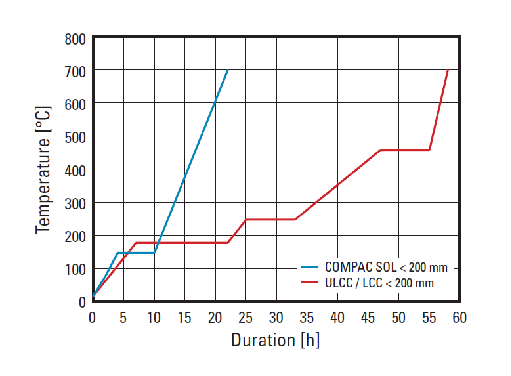
\includegraphics[width=0.7\textwidth]{figures/hucs.pdf}
        \caption{Exemplos de curvas de secagem comumente utilizadas. Retirado de \cite{rhi}}
        \label{fig:hucs}
   \end{figure}

   Portanto, o problema que o presente trabalho aborda é como usar ferramentas
   matemáticas para modelar os fenômenos de transporte de massa e calor que
   ocorrem durante a secagem para contribuir no entendimento desse complexo
   fenômeno e possibilitar que otimizações sejam realizadas tornando tal
   processo mais eficiente em termos de tempo e de consumo energético
   contribuindo para a redução dos custos financeiros e ambientais que tal
   processo inflige atualmente.
 
   A existência de ferramentas computacionais para a simulação de tal processo
   derivam de trabalhos baseados nos estudos de concretos de construção civil
   sujeitos a altas temperaturas em reatores nucleares ou em construções em
   incêndio \cite{bazant1978thermal, Abdel-Rahman1996, Gawin2004}. Esses modelos
   podem considerar inúmeros processos simultâneos, o que eleva sua
   complexidade. Sendo assim, um desafio abordado no presente trabalho é tentar
   usar simplificações que possibilitem o uso de tais ferramentas em aplicações
   refratárias.
   
\section{Objetivos}
    \subsection{Objetivo geral}
        
    Desenvolver e implementar um modelo numérico que considere o menor número
    possível de parâmetros para poder prever a secagem de materiais refratários
    monolíticos, utilizando o ensaio de termogravimetria (TGA) para realizar a
    validação da simulação numérica.
        
    \subsection{Objetivos específicos}
        
    \begin{itemize}
    \item Realizar uma revisão bibliográfica sobre as metodologias de otimização
      de curvas de secagem;
        
    \item Desenvolver um modelo capaz de simular os resultados do ensaio de
      termogravimetria utilizando apenas soluções \textit{open source};
        
    \item Realizar o \textit{benchmarking} do modelo com os dados do ensaio de
      termogravimetria (TGA);
        
    \item Testar o modelo para a otimização de uma curva de secagem.
    \end{itemize}
        
\section{Motivação}
Materiais refratários são fundamentais nas principais indústrias habilitadoras,
isto é, indústrias que fornecem maneiras de manufaturar outros materiais. No
caso, o processo siderúrgico, que é responsável por 5 \% \cite{Davis2018} da
liberação de CO$_2$ mundial anual está intimamente relacionado com a indústria
de materiais refratários. Tal relação é tamanha que a qualidade dos aços
produzidos dependem diretamente da qualidade do material refratário, que
permite, por exemplo, reduzir o teor de carbono das ligas. Além disso, embora os
avanços da área tenham reduzido consideravelmente a quantidade de refratário
consumida por tonelada de aço (chegando até o valor de 10kgs por tonelada de aço
no Japão \cite{Report2003}) esse valor é ainda expressivo e com potencial para redução em
diferentes mercados (como no mercado Chinês, onde estima-se um consumo de 23kgs
por tonelada de aço) \cite{refperton}.

   Nesse contexto, ampliar a vida útil dos refratários, diminuir o impacto
   ambiental de sua instalação e otimizar os tempos de manutenção podem ter
   efeitos determinantes tanto em aspectos sócio-ambientais como também
   consequências financeiras que permitam investimentos e avanços em novos
   materiais, gerando um processo contínuo de ganho de eficiência.

   A simulação do processo de secagem influencia em todos esses aspectos de
   maneira direta ou indireta, através da redução dos danos proporcionados pela
   pressão de vapor gerado no interior do material, e assim, ampliando a sua
   vida útil, agilizando a remoção da água física e quimicamente ligada,
   acelerando os processos de secagem e reduzindo o consumo de energia para o
   primeiro aquecimento e diminuindo as curvas iniciais de secagem, permitindo
   um ganho de eficiência no processo de manutenção dos equipamentos.

   Além dos ganhos de otimização, um maior entendimento dos processos
   simultâneos que ocorrem durante a secagem podem oferecer novos
   \textit{insights} para soluções que consigam garantir uma relação otimizada
   de permeabilidade e resistência mecânica do material, duas propriedades
   fundamentalmente inversamente proporcionais e que influenciam diretamente na
   curva de secagem a ser utilizada em cada material.


   \section{Resultados esperados} \label{results-esperados} Espera-se ao final
   desse projeto se ter um modelo capaz de simular numericamente o processo de
   secagem de um material refratário monolítico, validado através de ensaios
   baratos (sem necessitar de inúmeros termopares e transdutores de pressão) com
   um número reduzido de parâmetros. Através do uso de tal modelo, seria
   possível explorar metodologias para otimizar o processo de secagem dos
   materiais refratários monolíticos.

    
\section{Estrutura do trabalho}
    
Esta monografia encontra-se estruturada da seguinte forma:
    
\autoref{introducao} – apresenta a introdução do trabalho, seus objetivos, motivação e os resultados esperados;
    
\autoref{fundteorica} – descreve os conceitos de materiais refratários
monolíticos, apresentando suas principais características; avalia o estado da
arte das metodologias de controle e otimização empírica da remoção de água de
materiais refratários e por fim apresenta modelos gerais de secagem
    
\autoref{metodologia} – detalha os materiais e métodos utilizados no trabalho;
    
\autoref{results} – consiste na análise dos resultados obtidos tanto na
caracterização das propriedades necessárias ao modelo bem como dos testes
experimentais necessários para sua validação e por fim a comparação destes com
os resultados numéricos discutindo-se as razões de seu funcionamento e das
divergências terminando com a otimização de uma curva de secagem fictícia;

\autoref{conclusao} – apresenta a conclusão do trabalho e algumas sugestões para
trabalhos futuros.
    
Ao final da monografia encontram-se as referências bibliográficas utilizadas, um
apêndice apresentando detalhes do modelo matemático e uma explicação detalhada
do programa desenvolvido na linguagem Python \cite{python}.
